\chapter{Vector Bundles}\label{chapter:vector_bundles}

    The main reference for this chapter is \cite{bott_tu}.

\section{Tangent bundle}

    The tangent space, as introduced in Section \ref{section:tangent_space}, can also be introduced in a more natural way. Because it is the most important example of a vector bundle, tangent bundles are introduced first.
    \begin{construct}[Tangent bundle]\index{tangent!bundle}
        Let $M$ be an $n$-dimensional manifold with atlas $\{(U_i,\varphi_i)\}_{i\leq n}$. Construct for every open set $U$ an associated set $TU := U\times\mathbb{R}^n$ and construct for every smooth function $f$ an associated smooth function on $TU$, called the \textbf{differential} or \textbf{derivative} of $f$, by
        \begin{gather}
            \label{diff:T_function}
            Tf:U\times\mathbb{R}^n\rightarrow f(U)\times\mathbb{R}^n:(p,v)\mapsto(f(p),Df(p)v),
        \end{gather}
        where $Df(p):\mathbb{R}^n\rightarrow\mathbb{R}^n$ is the linear operator represented by the Jacobian matrix of $f$ at $p$.

        By applying this definition to the transition functions $\psi_{ji}$ one obtains a new set of functions \[\widetilde{\psi}_{ji}:=T\psi_{ji}:TU_i\rightarrow TU_j\] given by
        \begin{gather}
            \widetilde{\psi}_{ji}(\varphi_i(p),v) := \left(\varphi_j(p), D(\varphi_j\circ\varphi_i^{-1})(\varphi_i(p))v\right).
        \end{gather}
        Because the transition functions are diffeomorphisms, the associated Jacobians are invertible. This implies that the maps $\widetilde\psi_{ji}$ are elements of $\text{GL}(\mathbb{R}^n)$. The tangent bundle is then obtained by applying the fibre bundle construction theorem \ref{diff:fibre_bundle_construction_theorem} to the triple $(M, \mathbb{R}^n,\text{GL}(\mathbb{R}^n))$ together with the cover $\{U_i\}_{i\leq n}$ and the cocycle $\{\widetilde\psi_{ji}\}_{i,j\leq n}$.
    \end{construct}
    \begin{remark}[Topology]
        Although the tangent bundle is by construction bijective (as a set) to the Cartesian product $M\times\mathbb{R}^n$ or the disjoint union $\bigsqcup_{p\in M}T_pM$, this does not hold on the level of topologies. It is not equipped with the disjoint union topology.
    \end{remark}

    \newdef{Natural chart}{\index{natural!chart}\index{adapted!chart|see{natural chart}}
        The charts in the atlas on this bundle are sometimes called \textbf{natural charts} or \textbf{adapted charts} because the first $n$ coordinates are equal to the coordinates on the base space.
    }

    \newdef{Tangent space}{\index{tangent!space}
        Consider a point $p\in M$. The definition of the tangent space in the above setting is given by the fibre
        \begin{gather}
            T_pM := \pi_{TM}^{-1}(p).
        \end{gather}
        If one uses the natural charts to map $T_pM$ to the set $\varphi_i(p)\times\mathbb{R}^n$, it can be seen that $T_pM$ is isomorphic to $\mathbb{R}^n$ (as a vector space).
    }

    \begin{property}[Smooth structure]
        An atlas on $TM$ is given by the charts $(TU_i,\theta)$ with
        \begin{gather}
            \theta:TM\rightarrow\mathbb{R}^{2n}:(p, X)\mapsto(\varphi_i\circ\pi(p),X^1,\ldots,X^n),
        \end{gather}
        where $(U_i,\varphi_i)$ is a around $p\in M$ with local coordinates $(x^1,\ldots,x^n)$ such that $X$ can be expressed as $X^i\partial_i\in T_pM$.
    \end{property}

    \begin{property}[Dimension]
        Let $M$ be an $n$-dimensional manifold. Using the natural charts on $TM$ and the charts on $M$ one can see that $TM$ is locally isomorphic to $\mathbb{R}^{2n}$. This implies that
        \begin{gather}
            \dim TM = 2\dim M.
        \end{gather}
    \end{property}

    \begin{remark}[Physics]
        Now it is clear that the statement ``\textit{a vector is something that transforms like a vector}'', which one often hears in introductory physics courses, comes from the fact that \[\text{a vector }v\in T_pM\text{ is tangent to }\varphi_i(p)\text{ in a chart }(U_i,\varphi_i)\] if and only if \[D(\varphi_j\circ\varphi_i^{-1})(\varphi_i(p))v\text{ is tangent to }\varphi_j(p)\text{ in a chart }(U_j,\varphi_j).\]
    \end{remark}

    \newdef{Differential}{\index{differential}\label{diff:differential}
        The map $T$ defined in equation \eqref{diff:T_function} can be generalized to arbitrary smooth manifolds as the map $Tf:TM\rightarrow TN$, where the Jacobian now acts on the (linear) fibres. Furthermore, let $p\in U\subseteq M$ and let $V = f(U)$. By looking at the restriction of $Tf$ to $T_pM$, denoted by $T_pf$, one sees that it maps $T_pU$ to $T_{f(p)}V$ linearly.
    }

    \begin{property}
        The map $Tf:TM\rightarrow TN$ has the following properties\footnote{This turns the map $T$ into an endofunctor on the category of smooth manifolds. Hence, one can view $T$ as a ``functorial derivative''.}:
        \begin{itemize}
            \item $T$ preserves identities: $T\mathbbm{1}_M = \mathbbm{1}_{TM}$.
            \item Let $f,g$ be two smooth functions on smooth manifolds, then $T(f\circ g) = Tf\circ Tg$.
        \end{itemize}
    \end{property}

    \newdef{Rank}{\index{rank!of function}\label{diff:rank}
        Let $f:M\rightarrow N$ be a differentiable function between smooth manifolds. Using the fact that $Tf$ is fibrewise linear, the rank of $f$ at $p\in M$ is defined as the rank (in the sense of \ref{linalgebra:image_rank}) of the differential $Tf:T_pM\rightarrow T_{f(p)}N$.
    }

    \begin{theorem}[Inverse function theorem]\index{inverse function theorem}\label{diff:inverse_function_theorem}
        A smooth function $f:M\rightarrow N$ between smooth manifolds is a local diffeomorphism at $p\in M$ if and only if its differential $Tf:T_pM\rightarrow T_{f(p)}N$ is an isomorphism at $p$.
    \end{theorem}

    \newdef{Parallelizable manifold}{\index{parallelizable}
        A manifold is said to be parallelizable if its tangent bundle is trivial.
    }

    \newdef{Normal bundle}{\index{normal!bundle}
        Consider a smooth manifold $M$ with a submanifold $S$ and consider for every point $p\in S$ the tangent spaces $T_pS$ and $T_pM$. Since $T_pS$ is a subspace of $T_pM$, one can construct the quotient space $N_pS := T_pM/T_pS$. The normal bundle of $S$ in $M$ is defined as the vector bundle with fibres $N_pS$.
    }
    \newdef{Tubular neighbourhood}{\index{tubular neighbourhood}\label{diff:tubular_neighbourhood}
        Consider a smooth manifold $M$ with an embedded submanifold $S$. A tubular neighbourhood of $S$ in $M$ is a vector bundle $\pi:E\rightarrow S$ such that (an open neighbourhood of the zero section of) $E$ is diffeomorphic to an open neighbourhood of $S$ in $M$.
    }
    \begin{theorem}[Tubular neighbourhood theorem]\label{diff:tubular_neighbourhood_theorem}
        Every embedded submanifold admits a tubular neighbourhood, namely its normal bundle. Furthermore, all tubular neighbourhoods are diffeomorphic.
    \end{theorem}
    \begin{result}[Submanifolds and NDR pairs]\label{diff:ndr_submanifold}
        Consider a smooth manifold $M$ and a submanifold $S$. The pair $(M,S)$ is an NDR pair \ref{topology:ndr_pair_homology}. In particular, consider a smooth fibre bundle $\pi:E\rightarrow B$. If $\pi$ admits a global section, one can embed $B$ in $E$ as a submanifold and hence the pair $(E,B)$ is an NDR pair.
    \end{result}

\section{Vector bundles}

    Instead of restricting the typical fibre to be a Euclidean space with the same dimension as the base manifold, one can generalize the construction of the tangent bundle in the following way:
    \begin{construct}[Vector bundle]\index{vector!bundle}\index{rank!of vector bundle}\label{diff:vector_bundle_construction}
        \nomenclature[S_Vect]{$\textbf{Vect}(X)$}{category of vector bundles over a topological space $X$}
        Consider an $n$-dimensional manifold $M$ with atlas $\{(U_i,\varphi_i)\}_{i\leq n}$ together with a cocycle $\{g_{ji}:U_i\cap U_j\rightarrow G\}_{i,j\leq n}$ with values in a group $G$ and a representation $\rho:G\rightarrow\text{GL}(V)$ on a (finite-dimensional) vector space $V$. A bundle can then be constructed using Construction \ref{diff:fibre_bundle_construction_theorem}. The dimension of the typical fibre $V$ is called the \textbf{rank} of the vector bundle.
    \end{construct}
    \begin{remark}
        As was also the case for tangent bundles, the choice of charts on $E$ is not random. To preserve the structure of fibres, the use of the natural charts is imperative.
    \end{remark}

    \begin{example}[Line bundle]\index{line!bundle}\index{wave!function}
        A vector bundle with a one-dimensional fibre. A common example is the $\mathbb{C}$-line bundle over some smooth manifold whose sections in quantum mechanics correspond to the wave functions describing a given system. See Section \ref{section:geometric_quantization} on geometric quantization for more information.
    \end{example}

\subsection{Sections}

    \newdef{Frame}{\index{frame}\label{diff:frame}
        A frame of a vector bundle $E$ is a tuple $(s_1,\ldots,s_n)$ of smooth sections such that $(s_1(b),\ldots,s_n(b))$ is a basis for the fibre $\pi^{-1}(b)$ for all $b\in B$.
    }
    \begin{property}\label{diff:trivial_vector_bundle}
        A vector bundle is trivial if and only if there exists a global frame.
    \end{property}

    \begin{theorem}[Serre \& Swan]\index{Serre-Swan}\label{diff:serre_swan}
        The set of all smooth sections of a vector bundle with base space $M$ is a finitely-generated projective $C^\infty(M)$-module.
    \end{theorem}

    \begin{property}[Zero section]\label{diff:zero_section}
        The zero section $s_0$ of a vector bundle $E\rightarrow M$ is the map that assigns to every point $p\in M$ the zero vector of the associated vector space $E_p$. For every smooth vector bundle $\pi:E\rightarrow M$ one can embed the base manifold $M$ in the bundle $E$ through the zero section $s_0:M\rightarrow E$. The complement of the image of this section is often denoted by $E_0$.
    \end{property}

\subsection{Whitney sums}

    \newdef{Whitney sum}{\index{Whitney!sum}\index{direct!sum}
        Consider two vector bundles $E,E'$ with typical fibres $W,W'$ over the same base manifold. One can construct a new vector bundle $E\oplus E'$ by taking the typical fibre to be the direct sum $W\oplus W'$, i.e. the fibre over $p$ is given by $W_p\oplus W_p'$. This operation is called the Whitney sum or \textbf{direct sum} of vector bundles.
    }

    Property \ref{linalgebra:complement} from linear algebra can be generalized in the following way:
    \begin{property}
        Let $M$ be a paracompact Hausdorff space and let $E$ be a vector bundle over $M$. Every vector subbundle $F$ of $E$ admits an orthogonal complement $F^\perp$.
    \end{property}
    \begin{property}\label{diff:hausdorff}
        Let $M$ be a compact Hausdorff space. Every vector bundle $E$ over $M$ admits a complementary vector bundle $E^c$ such that $E\oplus E^c \cong M\times\mathbb{R}^n$ for some $n\in\mathbb{N}$.
    \end{property}

    \newdef{Stable isomorphism}{\index{stable!isomorphism}\label{diff:stable_isomorphism}
        Two vector bundles $E,E'$ over a base space $M$ are said to be stably isomorphic if there exist integers $m,n\in\mathbb{N}$ such that
        \begin{gather}
            E \oplus (M\times\mathbb{R}^m)\cong E' \oplus (M\times\mathbb{R}^n).
        \end{gather}
    }

\subsection{Associated vector bundles}

    \begin{construct}[Associated vector bundle]\index{associated!vector bundle}\label{diff:associated_vector_bundle}
        Consider a representation \[\rho:\text{GL}(\mathbb{R}^n)\rightarrow\text{GL}(\mathbb{R}^l)\] together with the tangent bundle cocycle $\{t_{ji} := D(\psi_{ji})\circ\varphi_i\}_{i,j\leq n}$. The composite \[\rho\circ t_{ji}:U_i\cap U_j\xrightarrow{t_{ji}} \text{GL}(\mathbb{R}^n)\xrightarrow{\rho}\text{GL}(\mathbb{R}^l)\] is again a cocycle and can thus be used to define a new vector bundle on $M$ through Construction \ref{diff:fibre_bundle_construction_theorem}. The vector bundle $E\equiv\rho(TM)$ is called the associated (vector) bundle of the tangent bundle induced by $\rho$.
    \end{construct}

    \begin{example}[Contravariant vectors]\index{contravariant}
        By noting that the $k^{th}$ tensor power $\otimes^k$ induces a representation given by the tensor product of representations, one can construct the bundle of order-$k$ (contravariant) tensors $\otimes^k(TM)$.
    \end{example}
    \begin{example}[Cotangent bundle]\index{covariant}\index{co-!vector}\label{diff:cotangent_bundle}
        Another useful construction is given by the contragredient representation $A\mapsto (\rho^T)^{-1}=(\rho^{-1})^T$. The vector bundle constructed this way, where the cocycle is given by $(t_{ji}^T)^{-1}$, is called the cotangent bundle on $M$ and is denoted by $T^*M$. Elements of the fibres are called \textbf{covariant vectors} or \textbf{covectors}.
    \end{example}
    \begin{notation}
        A combination of the cocycle $t_{ji}$ and its dual $(t_{ji}^T)^{-1}$ can also be used to define the bundle of $(k,l)$-tensors on $M$. This bundle is denoted by $T^{(k,l)}M$.
    \end{notation}

    \newdef{Twisted bundle}{\index{twisting}
        Given a vector bundle $\pi:E\rightarrow M$ and a line bundle $\psi:L\rightarrow M$, one calls the tensor product $E\otimes L$ the ``$L$-twisted'' version of $E$. Often the vector bundle $E$ will be a bundle of $k$-forms such that one obtains the $L$-valued differential forms of Section \ref{section:vector_valued_forms} below.
    }

    For every vector bundle one can define a canonical line bundle:
    \begin{construct}[Determinant line bundle]\index{bundle!determinant}\index{determinant!line bundle|see{bundle, determinant}}\index{density}
        Consider a rank-$n$ vector bundle $\pi:E\rightarrow M$. The determinant map induces an associated line bundle $\det(\pi):\det(E):=\bigwedge^nE\rightarrow M$ where the transition functions on the fibres are given by the determinant of the transition functions of $E$. Bundles twisted by a determinant line bundle are called \textbf{densitized bundles}.
    \end{construct}
    \begin{example}[Canonical bundle]\index{bundle!canonical}\label{diff:canonical_bundle}
        Consider a smooth $n$-dimensional manifold $M$. The canonical (line) bundle of $M$ is given by $\det(T^*M)\equiv\bigwedge^nT^*M$, i.e. the determinant line bundle of the cotangent bundle of $M$.
    \end{example}

\subsection{Grassmann bundle}

    Looking at Property \ref{linalgebra:grassmannian_construction} and noting that $\text{GL}_n(\mathbb{R})$ is a Lie group, it is clear that one can endow the Grassmannian $\text{Gr}(k,\mathbb{R}^n)$ from Definition \ref{linalgebra:grassmannian} with a differentiable structure, thereby turning it into a smooth manifold. This allows the construction of a new bundle by applying the construction theorem \ref{diff:fibre_bundle_construction_theorem}. Because the Grassmannian is not a vector space, the resulting bundle will be a general fibre bundle and not a vector bundle.

    \begin{construct}[Grassmann bundle]\index{Grassmann!bundle}\label{diff:grassmann_bundle}
        One first defines a new set of transition functions
        \begin{gather}
            \psi_{ji}:(\varphi_i(p),V)\mapsto(\varphi_j(p),t_{ji}(p)\cdot V),
        \end{gather}
        where $\{t_{ji}\}_{i,j\leq n}$ is the tangent bundle cocycle. These transition functions can be used to create a new fibre bundle with typical fibre $\text{Gr}(k, \mathbb{R}^n)$. The fibre over a point $p\in M$ is the Grassmannian $\text{Gr}(k,T_pM)$ associated to the tangent space over $p$.

        By replacing the tangent bundle $TM$ by an arbitrary vector bundle $E$ (and accordingly replacing the cocycle $t$ with the cocycle of $E$) one can define the Grassmann bundle for a general vector bundle.
    \end{construct}
    \begin{notation}
        The Grassmann $k$-plane bundle of a vector bundle $E$ is denoted by $\text{Gr}(k,E)$.
    \end{notation}

    \newdef{Tautological bundle}{\index{tautological!bundle}\label{diff:tautological_bundle}
        Consider the Grassmannian $\text{Gr}(n,V)$ of an $(n+k)$-dimensional vector space $V$. The total space of the tautological $k$-bundle $\gamma_{n,k}$ is defined as the set of points $(W,w)$ where $W\in\text{Gr}(n,V)$ and $w\in W$. Local trivializations are constructed as follows:
        \begin{gather}
            \varphi_Z:\pi^{-1}(U)\rightarrow\text{Gr}(n,V)\times Z:(W,w)\mapsto (W,\text{proj}_Z(w)),
        \end{gather}
        where $\text{proj}_Z$ is the orthogonal projection onto the subspace $Z\in\text{Gr}(n,V)$. This bundle inherits a natural vector bundle structure from $V$.
    }

    \begin{definition}\index{Serre!twisting sheaf}
        Consider the tautological line bundle $J$ over a projective space $\mathbb{C}\mathbb{P}^n=\text{Gr}(1,\mathbb{C}^n)$. The dual line bundle $\hom(J, \mathbb{C})$ is often denoted by $\mathcal{O}_{\mathbb{CP}^n}(1)$ or $\mathcal{O}(1)$ and is sometimes called \textbf{Serre's twisting sheaf}. Tensor powers of this bundle are accordingly denoted by $\mathcal{O}_{\mathbb{CP}^n}(k)$. To also allow for factors of $J$ one can extend the notation to negative indices: $\mathcal{O}_{\mathbb{CP}^n}(-k)$, e.g. the tautological bundle is denoted by $\mathcal{O}_{\mathbb{CP}^n}(-1)$.
    \end{definition}

    \begin{property}[Euler sequence]\index{Euler!sequence}
        The dual bundle $\mathcal{O}_{\mathbb{CP}^n}(1)$ fits in a short exact sequence
        \begin{gather}
            0\longrightarrow\underline{\mathbb{C}}\longrightarrow\mathcal{O}_{\mathbb{CP}^n}(1)^{\oplus(n+1)}\longrightarrow T\mathbb{CP}^n\longrightarrow0,
        \end{gather}
        where $\underline{\mathbb{C}}$ denotes the trivial line bundle.
        \begin{proof}[Sketch of proof]
            Note that vector fields on $\mathbb{CP}^n$ can be obtained by pairing (coordinate-induced) basis vectors $\partial_i$ on $\mathbb{C}^{n+1}$ with linear functions on $\mathbb{C}^{n+1}$, i.e. with sections of $\mathcal{O}_{\mathbb{CP}^n}(1)$. The kernel of this map is given by the Euler vector field $\mathbb{E}:=x^i\partial_i$ and its scalar multiples.
        \end{proof}
    \end{property}

\section{Vector fields}

    \newdef{Vector field}{\index{vector field}
        A smooth section $s\in\Gamma(TM)$ of the tangent bundle. By the Serre-Swan theorem \ref{diff:serre_swan} the set of vector fields forms a $C^\infty(M)$-module.
    }
    \begin{notation}
        \nomenclature[S_zsymXM]{$\mathfrak{X}(M)$}{$C^\infty(M)$-module of vector fields on the manifold $M$}
        The set of all vector fields on a smooth manifold $M$ is often denoted by $\mathfrak{X}(M)$.
    \end{notation}

    \newdef{Index}{\index{index}
        Consider a smooth vector field $X$ on an $n$-dimensional smooth manifold $M$ and let $p\in M$ be an isolated zero of $X$. Because $p$ is isolated, one can find a small $(n-1)$-sphere around $p$ that does not contain any other zeroes of $X$. The index $\text{ind}_X(p)$ of $X$ at $p$ is defined as the degree \ref{topology:degree} of the function $f:S^{n-1}\rightarrow S^{n-1}:m\mapsto\frac{X(m)}{||X(m)||}$.
    }
    \begin{property}[Winding number]\index{winding number}
        The winding number of a vector field $X$ along a smooth curve $\gamma$ (where it is assumed that $X$ does not vanish on $\gamma$) is equal to the sum of indices of zeroes of $X$ lying inside $\gamma$.
    \end{property}

    \begin{theorem}[Poincar\'e-Hopf]\index{Poincar\'e-Hopf}
        Let $M$ be a compact smooth manifold and consider a vector field $X$ having only isolated zeroes.
        \begin{gather}
            \sum_{p:X(p)=0}\text{\emph{ind}}_X(p) = \chi(M),
        \end{gather}
        where $\chi$ denotes the Euler characteristic \ref{topology:euler_characteristic}.
    \end{theorem}

    An immediate consequence of the Poincar\'e-Hopf theorem is the following well-known result:
    \begin{theorem}[Hairy ball theorem]\index{hairy ball theorem}
        There exists no nowhere-vanishing vector field on an even-dimensional sphere $S^{2n}$.
    \end{theorem}

    \newdef{Pullback}{\index{pullback}
        Let $X$ be vector field on $N$ and let $\varphi:M\rightarrow N$ be a diffeomorphism. The pullback of $X$ along $\varphi$ is defined as
        \begin{gather}
            \label{diff:pullback}
            (\varphi^*X)_p := T\varphi^{-1}(X_{\varphi(p)}).
        \end{gather}
    }
    \newdef{Pushforward}{\index{pushforward}
        Let $X$ be a vector field on $M$ and let $\varphi:M\rightarrow N$ be a diffeomorphism. Using the differential $T\varphi$ one can define the pushforward of $X$ along $\varphi$ as
        \begin{gather}
            \label{diff:pushforward}
            (\varphi_*X)_{\varphi(p)} := T\varphi(X_p).
        \end{gather}
        This can be rewritten using the pullback as follows:
        \begin{gather}
            \label{diff:pullback_pushforward}
            \varphi_*X = (\varphi^{-1})^*X.
        \end{gather}
        Equivalently, one can define a vector field on $N$ by
        \begin{gather}
            (\varphi_*X)_q(f) := X_{\varphi^{-1}(q)}(f\circ\varphi)
        \end{gather}
        for all smooth functions $f:N\rightarrow\mathbb{R}$ and points $q\in N$.
    }

\subsection{Integral curves}

    \newdef{Integral curve}{\index{integral!curve}\label{diff:integral_curve}
        Let $X\in\mathfrak{X}(M)$ and let $\gamma:\ ]a,b[\rightarrow M$ be a smooth curve on $M$. $\gamma$ is said to be an integral curve of $X$ if
        \begin{gather}
            \gamma'(t) = X(\gamma(t))
        \end{gather}
        for all $t\in\ ]a,b[$ where $\gamma'(t) := T\gamma(t,1)$.

        This equation can be viewed as a system of ordinary differential equations. Using the Picard-Lindel\"of existence theorem \ref{diffeq:picard_lindelof}, together with the initial value condition $\gamma(0) = p$, one can find a unique maximal curve satisfying the defining equation \ref{diff:integral_curve}. This solution, denoted by $\gamma_p$, is called the \textbf{integral curve of $X$ through $p$}.
    }

    \newdef{Flow}{\index{flow}\label{diff:flow}
        Let $X\in\mathfrak{X}(M)$ and consider its integral curve $\gamma_p$ through a point $p\in M$. The function $\sigma_t$ defined by
        \begin{gather}
            \sigma_t(p) := \gamma_p(t),
        \end{gather}
        is called the flow of $X$ at time $t$. The \textbf{flow domain} is defined as the set
        \begin{gather}
            D(X) := \big\{(t,p)\in\mathbb{R}\times M\,\big\vert\,p\in M, t\in\ ]a_p,b_p[\big\},
        \end{gather}
        where $]a_p,b_p[$ is the maximal interval on which $\gamma_p(t)$ is defined.
    }
    \begin{property}
        Suppose that $D(X) = \mathbb{R}\times M$. The flow $\sigma_t$ has the following properties for all $s,t\in\mathbb{R}$:
        \begin{itemize}
            \item $\sigma_0 = \mathbbm{1}_M$,
            \item $\sigma_{s+t} = \sigma_s\circ\sigma_t$, and as a consequence
            \item $\sigma_{-t} = (\sigma_t)^{-1}$.
        \end{itemize}
        These three properties say that $\sigma_t$ is a bijective group action of the additive group of real numbers on $M$. This implies that $\sigma_t$ is indeed a \textbf{flow} in the general mathematical sense.
    \end{property}

    \newdef{Complete vector field}{\index{complete!vector field}\label{diff:complete_vector_field}
        A vector field $X$ is said to be complete if the flow domain for every flow is all of $\mathbb{R}\times M$.
    }

    \begin{property}
        The flow $\sigma_t$ of a vector field is of class $C^\infty$. If $X$ is complete, it follows from the previous property that every flow is a diffeomorphism from $M$ onto itself.
    \end{property}

    \begin{property}
        If the manifold $M$ is compact, every vector field $X\in\mathfrak{X}(M)$ is complete.
    \end{property}

    \begin{property}[Winding number]\index{winding number}
        The winding number of a vector field along a closed integral curve is 1.
    \end{property}

\subsection{Lie derivative}

    \newformula{Lie derivative for smooth functions}{\index{Lie!derivative}\label{diff:lie_derivative_functions}
        Let $X\in\mathfrak{X}(M)$ and let $f\in C^\infty(M)$. The Lie derivative of $f$ with respect to $X$ at $p\in M$ is defined as
        \begin{gather}
            \mathcal{L}_Xf(p) := \lim_{t\rightarrow0}\stylefrac{f(\gamma_p(t)) - f(p)}{t}.
        \end{gather}
        This closely resembles the definition of the ordinary derivative on Euclidean space.
    }

    \begin{formula}[$\dag$]\label{diff:lie_derivative_function}
        Working out the previous formula and rewriting it as an operator equality gives
        \begin{gather}
            \label{diff:lie_derivative_function_expansion}
            \mathcal{L}_X = \sum_kX_k\pderiv{}{x^k}.
        \end{gather}
        It is clear that this is just the vector field $X$ expanded in the basis \ref{diff:tangent_vector_partial}. One also recovers the behaviour of a tangent vector as a derivation. For smooth functions $f:M\rightarrow\mathbb{R}$ this gives
        \begin{gather}
            \mathcal{L}_Xf(p) = X_p(f).
        \end{gather}
    \end{formula}

    \newformula{Lie derivative for vector fields$^\dag$}{\label{diff:lie_derivative_vector_field}
        Let $X,Y\in\mathfrak{X}(M)$.
        \begin{gather}
            \mathcal{L}_XY(p) := \left.\deriv{}{t}(\sigma_t^*X)(\gamma_p(t))\right|_{t=0}.
        \end{gather}
    }
    \begin{property}\index{Lie!bracket}
        Let $X,Y\in\mathfrak{X}(M)$ be vector fields of class $C^k$. The Lie derivative has the following properties:
        \begin{itemize}
            \item $\mathcal{L}_XY$ is a vector field.
            \item \textbf{Lie bracket}: The Lie derivative of vector fields coincides with the commutator:
                \begin{gather}
                    \label{diff:lie_bracket}
                    \mathcal{L}_XY = [X, Y].
                \end{gather}
                The fact that this is indeed a derivation on $C^{k-1}(M, \mathbb{R})$ follows Schwarz's theorem \ref{calculus:schwarz_theorem}. This result shows that the Lie derivative on vector fields turns the space $\mathfrak{X}(M)$ into a real Lie algebra.
            \item The previous point also implies that the Lie derivative is antisymmetric:
                \begin{gather}
                    \label{diff:lie_derivative_antisymmetry}
                    \mathcal{L}_XY = -\mathcal{L}_YX.
                \end{gather}
        \end{itemize}
    \end{property}

    \newdef{Holonomic basis}{\index{holonomic!basis}
        Consider a smooth manifold $M$ and an open subset $U\subseteq M$. A local frame $\{e_i\}_{i\leq\dim(M)}$ for $TU$ is said to be holonomic if all the Lie derivatives vanish on $U$:
        \begin{gather}
            \mathcal{L}_{e_i}e_j = 0.
        \end{gather}
        Equivalently, a basis is holonomic if the associated structure coefficients of the Lie algebra $\mathfrak{X}(M)$ vanish on $U$.
    }
    \begin{property}
        For every holonomic basis there exists a coordinate system on $M$ such that the basis coincides with the coordinate-induced basis.
    \end{property}

\subsection{Frobenius's theorem}

    \newdef{Distribution}{\index{distribution!of $k$-planes}\label{diff:distribution}
        A smooth section of the Grassmann $k$-plane bundle \ref{diff:grassmann_bundle}.
    }

    \begin{definition}[Integrable]\index{integrable!manifold}
        Let $M$ be a smooth manifold and let $W\in\Gamma(\text{Gr}(k, TM))$ be a distribution of $k$-planes. A submanifold $N\subseteq M$ is said to integrate $W$ with initial condition $p_0\in M$ if for every $p\in N$ one has that $W(p) = T_pN$ and $p_0\in N$. $W$ is said to be integrable if there exists such a submanifold $N$.
    \end{definition}
    \begin{property}\index{leaf}\index{foliation}
        If a distribution on $M$ is integrable, $M$ can be written as the (disjoint) union of maximal connected integrable manifolds. These submanifolds are also called the \textbf{leaves} of the distribution (the decomposition in leaves defines a \textit{foliation}).
    \end{property}

    \newdef{Frobenius's integrability condition}{
        A distribution $W$ on a smooth manifold $M$ is said to satisfy the Frobenius integrability condition on an open set $U\subseteq M$ if for every two vector fields $X, Y$ defined on $U$, such that $X(p)\in W(p)$ and $Y(p)\in W(p)$ for all $p\in U$, the Lie bracket $[X,Y](p)$ is also an element of $W(p)$ for all $p\in U$.
    }
    \begin{theorem}[Frobenius's integrability theorem]\index{Frobenius!integrability theorem}\label{diff:frobenius}
        Let $W$ be a distribution over a smooth manifold $M$. $W$ is integrable if and only if it satisfies the Frobenius integrability condition.
    \end{theorem}

\section{Differential \texorpdfstring{$k$}{k}-forms}\label{section:forms}

    \newdef{Differential form}{\index{differential form}
        \nomenclature[S_zsymOmegak]{$\Omega^k(M)$}{$C^\infty(M)$-module of differential $k$-forms on the manifold $M$.}
        A differential $k$-form is a map
        \begin{gather}
            \omega:T^kM\rightarrow\mathbb{R}
        \end{gather}
        such that the restriction of $\omega$ to each fibre of the bundle $T^kM$ is multilinear and antisymmetric.

        The space of all differential $k$-forms on a manifold $M$ is denoted by $\Omega^k(M)$. Just like $\mathfrak{X}(M)$, it forms a $C^\infty(M)$-module. The space $\Omega^0(M)$ is defined as the space of smooth functions $C^\infty(M)$.
    }
    Differential forms can also be constructed as sections of an associated vector bundle \ref{diff:associated_vector_bundle}:
    \begin{adefinition}
        Consider the representation \[\rho_k:\text{GL}(\mathbb{R}^{m*})\rightarrow\text{GL}(\Lambda^k\mathbb{R}^{m*}): A\mapsto A\wedge\cdots\wedge A.\] This representation induces an associated vector bundle $\rho_k(\pi_{T^*M})$ of the cotangent bundle on $M$. A differential $k$-form is then given by a section of $\rho_k(\pi_{T^*M})$:
        \begin{gather}
            \Omega^k(M) := \Gamma(\rho_k(\pi_{T^*M})).
        \end{gather}
    \end{adefinition}

    \begin{construct}[Exterior algebra]
        One can construct a Grassmann algebra \ref{vector:exterior_algebra} by equipping the graded vector space
        \begin{gather}
            \Omega^\bullet(M) := \bigoplus_{k\geq0}\Omega^k(M)
        \end{gather}
        with the wedge product of differential forms which is induced by the wedge product on $\Lambda^k\mathbb{R}^m$. This graded algebra is associative, graded-commutative and unital with the constant function $1\in C^{\infty}(M)$ as the identity element.
    \end{construct}

    \newdef{Pullback}{\index{pullback}\label{forms:pullback}
        Let $f:M\rightarrow N$ be a smooth function between smooth manifolds and let $\omega$ be a differential $k$-form on $N$. The pullback of $\omega$ by $f$ is defined as
        \begin{gather}
            f^*(\omega) := \omega\circ f_*.
        \end{gather}
        This defines a map $f^*:\Omega^\bullet(N)\rightarrow\Omega^\bullet(M)$.
    }
    \newdef{Pushforward}{\index{pushforward}\label{forms:pushforward}
        Let $f:M\rightarrow N$ be a diffeomorphism between smooth manifolds and let $\omega$ be a differential $k$-form on $M$. The pushforward of $\omega$ by $f$ is defined as
        \begin{gather}
            f_*(\omega) := \omega\circ (f^{-1})_*.
        \end{gather}
    }
    \begin{remark*}
        Note that the pushforward of differential $k$-forms is only defined for diffeomorphisms, in contrast to pullbacks which only require smooth functions. This also explains why differential forms are the most valuable elements in differential geometry. Vector fields cannot even be pulled back by general smooth maps.
    \end{remark*}

    \newformula{Dual basis}{\index{basis}\label{diff:basis}
        Consider the coordinate basis from definition \ref{diff:tangent_vector_partial} for the tangent space $T_pM$. From this set one can construct a natural dual basis for the cotangent space $T_p^*M$ using the natural pairing:
        \begin{gather}
            \left\langle\pderiv{}{x^i}, dx^j\right\rangle = \delta_i^j.
        \end{gather}
        It should be noted that $dx^i$ is not just a notation. In the next section it will be shown that these basis vectors can be obtained by applying the ''exterior derivative'' to the coordinate functions $x^i$.
    }

\subsection{Exterior derivative}

    \newdef{Exterior derivative}{\index{exterior!derivative}\index{differential|seealso{exterior derivative}}\label{diff:exterior_derivative}
        The exterior derivative $d_k$ is a map constructed on the graded algebra of differential $k$-forms:
        \begin{gather}
            d_k:\Omega^k(M)\rightarrow\Omega^{k+1}(M).
        \end{gather}
        For $k=0$ it is defined by
        \begin{gather}
            \label{diff:function_derivative}
            df := \sum_{i=1}^n\pderiv{f}{x_i}dx_i
        \end{gather}
        The object $df\in\Omega^1(M)$ is often called the \textbf{differential} of $f$. This formula can be generalized to higher degree forms as follows:
        \begin{gather}
            d(fdx_{i_1}\wedge\cdots\wedge dx_{i_k}) := df\wedge dx_{i_1}\wedge\cdots\wedge dx_{i_k}.
        \end{gather}
    }
    \remark{Formula \ref{diff:function_derivative} should be compared with the (informal) formula for the differential of a function that is often used in physics. The main difference is that here the quantities $dx^i$ are not infinitesimal quantities but vectors of unit norm.}

    \begin{property}\index{Leibniz!rule}\label{diff:exterior_derivative_properties}
        The exterior derivatives satisfy the following properties for all $k\geq0$:
        \begin{itemize}
            \item For all $\omega\in\Omega^k(M)$:
                \begin{gather}
                    d_k\circ d_{k+1} = 0.
                \end{gather}
            \item $d_k$ is an $\mathbb{R}$-linear map.
        \end{itemize}
        These two items say that $(\Omega^\bullet(M),d)$ is not just a graded algebra, but in fact a dg-algebra \ref{homalg:dg_algebra}.
        \begin{itemize}
            \item \textbf{Graded Leibniz rule} (hence $d$ is a graded derivation):
                \begin{gather}
                    d(\omega_1\wedge\omega_2) = d\omega_1\wedge\omega_2 + (-1)^j\omega_1\wedge d\omega_2
                \end{gather}
                where $\omega_1\in\Omega^j(M)$ and $\omega_2\in\Omega^k(M)$.
            \item \textbf{Naturality}: If $f\in C^\infty(M)$, then $f^*(d\omega) = d(f^*\omega)$.
        \end{itemize}
    \end{property}

    \begin{remark}[$\dag$]\index{gradient}\index{rotor}\index{divergence}\label{diff:vector_calculus}
        The gradient, rotor (curl) and divergence from standard vector calculus\footnote{See Section \ref{section:nabla}.} can be rewritten using exterior derivatives as follows: Let $\mathbf{f} := (f_1,f_2,f_3)$ with $f_i$ smooth for every $i$ and let $f$ be a smooth function. Denote the canonical isomorphism between $\mathbb{R}^3$ and $\mathbb{R}^{3*}$ by $\sim$.
        \begin{align}
            \sim df &= \nabla f \\
            \sim (\ast d\alpha) &= \nabla\times\mathbf{f} \\
            \ast d\omega &= \nabla\cdot\mathbf{f}
        \end{align}
        The properties in section \ref{vector:mixed_properties} now follow from the identity $d^2 = 0$.
    \end{remark}

    \begin{example}
        Let $f\in C^\infty(M, \mathbb{R})$ and let $\gamma$ be a curve on $M$. From the definition \ref{diff:basis} of the basis $\{dx_k\}_{k\leq n}$ one obtains the following result:
        \begin{gather}
            \langle df(x), \gamma'(t) \rangle = \sum_k \pderiv{f}{x_k}(x)\gamma_k'(t) = (f\circ\gamma')(t).
        \end{gather}
    \end{example}

    \begin{example}
        An explicit formula for the exterior derivative of a k-form $\Phi$ is
        \begin{align}
            d\Phi(X_1,\ldots, X_{k+1}) = \sum_{i=1}^{k+1} &(-1)^{i+1} X_i(\Phi(X_1,\ldots, \hat{X}_i,\ldots, X_{k+1}))\nonumber\\
            \label{diff:k_form_exterior_derivative}
            &+\sum_{i<j} (-1)^{i+j}\Phi([X_i, X_j], X_1,\ldots, \hat{X}_i,\ldots, \hat{X}_j,\ldots, X_{k+1})
        \end{align}
        where $\hat{X}$ means that this argument is omitted.
    \end{example}

\subsection{Lie derivative}

    \newformula{Lie derivative of differential forms}{\index{Lie!derivative}\label{diff:lie_derivative_forms}
        \begin{gather}
            \mathcal{L}_X\omega(p) := \lim_{t\rightarrow0}\stylefrac{\sigma_t^*\omega - \omega}{t}(p)
        \end{gather}
    }

    \begin{formula}[Lie derivative of smooth functions]
        Using the definition of the exterior derivative of smooth functions \ref{diff:function_derivative} and the definition of the dual basis \ref{diff:basis}, one can rewrite the Lie derivative \ref{diff:lie_derivative_function_expansion} as
        \begin{gather}
            Xf(p) = df_p(X(p)).
        \end{gather}
    \end{formula}

    \begin{property}
        The Lie derivative has the following Leibniz-type property with respect to differential forms (this follows from equations \ref{diff:k_form_exterior_derivative} and \ref{diff:lie_bracket}):
        \begin{gather}
            \mathcal{L}_X(\omega (Y)) = (\mathcal{L}_X\omega)(Y) + \omega(\mathcal{L}_XY)
        \end{gather}
        where $X, Y$ are two vector fields and $\omega$ is a 1-form.
    \end{property}

\subsection{Interior product}

    \newdef{Interior product}{\index{interior!product}\label{diff:interior_derivative}
        Aside from the differential (exterior derivative) one can also define another operation on the algebra of differential forms:
        \begin{gather}
            \iota_X:(\iota_X\omega)(v_1,\ldots,v_{k-1})\mapsto\omega(X,v_1,\ldots,v_{k-1}).
        \end{gather}
        This antiderivation of degree $-1$ is called the \textbf{interior product} or \textbf{interior derivative}. It can be seen as a generalization of the contraction map \ref{vector:contraction}.
    }
    \begin{notation}
        In certain situations the above notation might become cumbersome. For this reason the notation $X\intmul\omega$ is frequently used.
    \end{notation}

    \newformula{Cartan's magic formula\footnotemark}{\index{Cartan!magic formula}\label{diff:cartan_magic_formula}
        \footnotetext{Sometimes called \textbf{Cartan's (infinitesimal) homotopy formula}.}
        Let $X$ be a vector field and let $\omega$ be a differential $k$-form. The Lie derivative of $\omega$ along $X$ is given by the following formula:
        \begin{gather}
            \mathcal{L}_X\omega = \iota_X(d\omega) + d(\iota_X\omega).
        \end{gather}
    }

\subsection{Lie derivative of tensor fields}

    \newformula{Lie derivative of tensor fields}{
        By comparing the definitions of the Lie derivatives of vector fields \ref{diff:lie_derivative_vector_field} and differential forms \ref{diff:lie_derivative_forms}, one can see that both definitions are identical upon replacing $X$ by $\omega$. This leads to the following definition of the Lie derivative of a general tensor field $\mathcal{T}\in\Gamma(T^{(k, l)}M)$:
        \begin{gather}
            \mathcal{L}_X\mathcal{T}(p) := \left.\deriv{}{t}\sigma_t^*\mathcal{T}(\gamma_p(t))\right|_{t=0}.
        \end{gather}
    }

    \newadef{Lie derivative of tensor fields}{
        The Lie derivative of tensor fields can also be defined as the unique differential operator satisfying the following axioms:
        \begin{enumerate}
            \item $\mathcal{L}_X$ coincides with $X$ on $C^\infty(M)$.
            \item $\mathcal{L}_X$ satisfies the Leibniz rule with respect to tensor products.
            \item $\mathcal{L}_X$ satisfies the Leibniz rule with respect to the contraction of forms and vector fields.
            \item $\mathcal{L}_X$ commutes with the exterior derivative.
        \end{enumerate}
    }

    \begin{property}
        Every derivation $D$ of the tensor algebra can be decomposed as
        \begin{gather}
            D = \mathcal{L}_X + S
        \end{gather}
        for some vector field $X$ and some endomorphism $S$.
    \end{property}

\subsection{Vector-valued differential forms}\label{section:vector_valued_forms}

    \newdef{Vector-valued form}{\index{differential form!vector-valued}
        Consider a vector space $V$ and let $E\rightarrow M$ be a vector bundle with typical fibre $V$. A vector-valued differential form on $M$ can be defined in two ways: One can define a vector-valued $k$-form as a map $\omega:\Gamma(T^kM)\rightarrow V$. However, a more general definition is based on sections of an associated bundle:
        \begin{gather}
            \Omega^k(M; E) := \Gamma(E\otimes\Lambda^kT^*M).
        \end{gather}
        The latter construction could also be called a ``vector bundle-valued differential form''.
    }

    \begin{construct}[Wedge product]\index{wedge!product}\label{diff:vector_valued_wedge}
        Let $\omega\in\Omega^p(M; E_1)$ and $\nu\in\Omega^q(M; E_2)$. The wedge product of these differential forms is defined as follows:
        \begin{gather}
            \omega\wedge\nu(v_1,\dots,v_{p+q}) := \stylefrac{1}{p!q!}\sum_{\sigma\in S_{p+q}}\sgn(\sigma)\omega(v_{\sigma(1)},\ldots, v_{\sigma(p)})\otimes\nu(v_{\sigma(p+1)},\ldots,v_{\sigma(q)}).
        \end{gather}
        This is a direct generalization of the formula for the wedge product of ordinary differential forms, where the scalar product (product in the algebra $\mathbb{R}$) is replaced by the tensor product (product in the tensor algebra). It should be noted that the result of this operation is not a section of any of the original bundles $E_1$ or $E_2$, but rather of the product bundle $E_1\otimes E_2$.
    \end{construct}

    \begin{construct}[Exterior derivative]\label{diff:twisted_differential}
        The definition of an exterior derivative on $E$-valued differential forms is more involved than in the case of ordinary forms. The logical thing to do would be defining a derivative through the Leibniz formula. However, without further structure on $E$ there is no natural way of differentiating sections of $E$.

        If $E$ is flat, i.e. if its transition functions are locally constant, one can choose a frame of sections $e^i:U\rightarrow E|_U$ induced by the trivializing maps $E|_U\rightarrow U\times\mathbb{R}^n$. Locally, one can then express any $E$-valued differential form as $\omega|_U=\sum_i\omega_i\otimes e^i$ where the $\omega_i$ are ordinary differential forms. After setting $de^i:=0$ one can again define an exterior derivative through the Leibniz formula.
    \end{construct}
    \begin{remark}
        It should be noted that the definition of $d$ depends on the choice of trivialization since the sections $e^i$ depend on this choice.
    \end{remark}

    \newdef{Lie algebra-valued form}{\index{differential form!Lie algebra-valued}
        A vector-valued differential form where the vector space $V$ is equipped with a Lie algebra structure.
    }
    \newformula{Wedge product}{\index{wedge!product}\label{diff:lie_algebra_valued_wedge}
        Let $\omega\in\Omega^p(M;\mathfrak{g})$ and $\nu\in\Omega^q(M; \mathfrak{g})$ where $\mathfrak{g}$ is a Lie algebra. The wedge product of these differential forms is defined as follows:
        \begin{gather}
            [\omega\wedge\nu](v_1,\ldots,v_{p+q}) := \stylefrac{1}{p!q!}\sum_{\sigma\in S_{p+q}}\sgn(\sigma)[\omega(v_{\sigma(1)},\ldots, v_{\sigma(p)}),\nu(v_{\sigma(p+1)},\ldots,v_{\sigma(q)})]
        \end{gather}
        where $[\cdot,\cdot]$ denotes the Lie bracket on $\mathfrak{g}$.
    }

    \begin{formula}
        Let $\{e_\mu\}_{\mu\leq\dim(\mathfrak{g})}$ be a basis for the Lie algebra $\mathfrak{g}$. One can write any Lie algebra-valued differential forms as $\phi = \phi^\mu \otimes e_\mu$ and $\psi = \psi^\nu \otimes e_\nu$, where $\phi^\mu$ and $\psi^\nu$ are ordinary differential forms. The above formula for the wedge product can now be rewritten more elegantly as
        \begin{gather}
            [\phi\wedge\psi] = (\phi^\mu\wedge\psi^\nu)\otimes[e_\mu, e_\nu]
        \end{gather}
        where $\wedge$ is the wedge product on $\Omega^\bullet(M)$ and $[\cdot,\cdot]$ denotes the Lie bracket on $\mathfrak{g}$.
    \end{formula}
    \begin{result}[Graded algebra]
        Using the above formula it is easy to verify a number of properties similar to the ones of ordinary differential forms. As an example the analogue of the graded-commutativity property on $\Omega^\bullet(M)$ is given:
        \begin{gather}
            [\phi\wedge\psi] = (-1)^{pq+1}[\psi\wedge\phi]
        \end{gather}
        where $\phi\in\Omega^p(M; \mathfrak{g})$ and $\psi\in\Omega^q(M; \mathfrak{g})$. Here the extra factor $-1$ arises due to the antisymmetry of the Lie bracket.

        Analogously, one can prove that the Lie algebra-valued wedge product satisfies a graded Jacobi-type identity:
        \begin{gather}
            (-1)^{pr}[\phi\wedge[\psi\wedge\theta]] + (-1)^{pq}[\psi\wedge[\theta\wedge\phi]] + (-1)^{qr}[\theta\wedge[\phi\wedge\psi]] = 0
        \end{gather}
        where $\theta\in\Omega^r(M; \mathfrak{g})$.
    \end{result}

\chapter{Integration Theory}\label{chapter:integration_manifolds}

For the theory on measure spaces and Lebesgue integration see chapter \ref{chapter:lebesgue}.

\section{Orientation}
	\newdef{Orientation}{\index{orientation}\index{volume}
		Similar to definition \ref{tensor:orientation} we can define an orientation on a differentiable manifold $M$. First we modify the definition of the volume element a little bit. A \textbf{volume form} on $M$ is a nowhere-vanishing top-dimensional differential form $\text{Vol}\in\Omega^n(M)$ where $n = \dim(M)$. The definition of an orientation is then equivalent to that in \ref{tensor:orientation}.
		
		An \textbf{oriented atlas} is given by all charts of $M$ for which the pullback of the Euclidean volume form is a positive multiple of $\text{Vol}$. This also means that the transition functions have a positive Jacobian determinant\footnotemark. The existence of a volume form turns a differentiable manifold into an \textbf{orientable manifold}.
		\footnotetext{This gives the equivalence with definition \ref{diff:orientable_structure} using $G$-structures.}
		
		Alternatively an orientable manifold with volume form $\omega$ is said to be \textbf{positively oriented} if $\omega(v_1, ..., v_n)>0$ where $(v_1, ..., v_n)$ is a basis for $T_pM$.
	}
	
	\begin{example}\index{determinant}
		Let $M=\mathbb{R}^n$. The canonical Euclidean volume form is given by the determinant map
		\begin{equation}
			\det:(u_1, ..., u_n)\mapsto\det(u_1, ..., u_n)
		\end{equation}
		where the $u_n$'s are expressed in the canonical basis $(e_1, ..., e_n)$. The name `volume form' is justified by noting that the determinant map gives the signed volume of the n-dimensional parallelotope spanned by the vectors $\{u_1, ..., u_n\}$.
	\end{example}
	
	\begin{property}
		Let $\omega_1, \omega_2$ be two volume forms on $M$. Then there exists a smooth function $f$ such that \[\omega_1 = f\omega_2\] Furthermore, the sign of this function is constant on every connected component of $M$.
	\end{property}

\section{Integration of top-dimensional forms}\index{Lebesgue!integral}\index{measure}

	\newdef{Measure zero}{
		A subset $U\subset M$ of an orientable manifold is said to be of measure zero if it is the countable union of inverse images of null sets in $\mathbb{R}^n$.
	}
	
	\newdef{Integrable form}{
		A differential form is said to be integrable if its components with respect to any basis of $\Omega^k(M)$ are Lebesgue integrable on $\mathbb{R}^n$.
	}

	\begin{formula}[Compact support]
		Let $\omega$ be a top-dimensional form on $M$ with compact support on $U\subset M$.
		\begin{equation}
			\label{forms:integration_compact_support}
			\int_M\omega = \int_U\omega = \int_{-\infty}^{+\infty}\cdots\int_{-\infty}^{+\infty}\omega_{12...n}(x)dx^1dx^2...dx^n
		\end{equation}
		This integral is well defined because under a (orientation preserving) change of coordinates the component $\omega_{1...n}$ transforms as $\omega'_{1...n} = J\omega_{1...n}$ where $J$ is the Jacobian determinant. Inserting this in the integral and replacing $dx_i$ by $dx'_i$ then gives us the well-known change-of-variables formula from Lebesgue integration theory.
	\end{formula}

	\begin{formula}[General]
		Let $\omega$ be a top-dimensional form on $M$ and let $\{\varphi_i\}_i$ be a partition of unity\footnotemark\ subordinate to an atlas on $M$.
		\footnotetext{This always exists if we require $M$ to be paracompact. See definition \ref{topology:partition_of_unity} and property \ref{topology:paracompact_partition_unity}.}
		\begin{equation}
			\label{forms:integration}
			\int_M\omega = \sum_i\int_M\varphi_i\omega
		\end{equation}
		where the integrals on the right-hand side are defined as in equation \ref{forms:integration_compact_support}.
	\end{formula}
	
	\newprop{Compact manifolds}{
		Let $M$ be a smooth compact manifold. Because every continuous form on $M$ is obviously compactly supported all continuous forms are integrable on $M$.
	}
	\newprop{Pullback}{
		Let $f:M\rightarrow N$ be an orientation-preserving diffeomorphism.
		\begin{equation}
			\int_Mf^*\omega = \int_N\omega
		\end{equation}
	}
	
	\begin{notation}
		Because the integral of differential forms satisfies properties similar to the ones listed in \ref{lebesgue:general_properties} we introduce the following notation:
		\begin{equation}
			\int_M\omega = \langle M, \omega \rangle
		\end{equation}
	\end{notation}
	
\section{General integration}

\section{Stokes' theorem}	

	\begin{theorem}[Stokes' theorem]\index{Stokes!theorem for differential forms}
		Let $\Sigma$ be an orientable smooth manifold. Denote the boundary of $\Sigma$ by $\partial\Sigma$. Let $\omega$ be a differential $k$-form on $\Sigma$. We have the following equality:
		\begin{equation}
			\label{forms:theorem:stokes_theorem}
			\boxed{\int_{\partial\Sigma}\omega = \int_\Sigma d\omega}
		\end{equation}
	\end{theorem}
	\begin{result}
		The Kelvin-Stokes theorem \ref{vectorcalculus:stokes_theorem}, the divergence theorem \ref{vectorcalculus:divergence_theorem} and Green's identity \ref{vectorcalculus:green_indentity} are immediate results of this (generalized) Stokes' theorem.
	\end{result}

\section{de Rham Cohomology}\index{cochain}\index{de Rham!cohomology}

	Now we can also give a little side note about why the de Rham cohomology groups \ref{forms:de_rham_cohomology} really form a cohomology theory. For this we need some concepts from homology which can be found in section \ref{section:homology}. Let $M$ be a compact differentiable manifold and let $\{\lambda_i:\Delta^k\rightarrow M\}$ be the set of singular $k$-simplexes on $M$.
	
	Now suppose that we want to integrate over a singular $k$-chain $C$ on $M$, i.e. $C = \sum_{i=0}^ka_i\lambda_i$. Formula \ref{forms:integration} says that we can pair the $k$-form $\omega$ and the chain $C$ such that they act as duals to each other (hence $p$-forms are also called $p$-\textbf{cochains}), producing a real number\footnote{This requires the chain group to have real coefficients instead of integer coefficients as is mostly used in homology.}:
	\begin{equation}
		\langle\cdot,C\rangle:\Omega^n(M)\rightarrow\mathbb{R}:\omega\mapsto\int_C\omega = \sum_{i=0}^ka_i\int_{\Delta_k}\lambda_i^{*}\omega
	\end{equation}
	where $\lambda_i^*$ pulls back $\omega$ to $\Delta^k$ which is a subset of $\mathbb{R}^k$ as required. Now Stokes' theorem \ref{forms:theorem:stokes_theorem} tells us that
	\begin{equation}
		\int_Cd\omega = \int_{\partial C}\omega
	\end{equation}
	Using the pairing $\langle\cdot,\cdot\rangle$ this becomes
	\begin{equation}
		\langle d\omega, C\rangle = \langle \omega, \partial C\rangle
	\end{equation}
	The operators $d$ and $\partial$ can thus be interpreted as formal adjoints. After checking (again using Stokes' theorem) that all chains $C$ and cochains $\omega$ belonging to the same equivalence classes $[C]\in H_k(M, \mathbb{R})$ and $[\omega]\in H^k(M, \mathbb{R})$ give rise to the same number\footnote{Suppose that $A, B\in [C]$ and $\phi, \chi\in[\omega]$ then $\langle \phi, A \rangle = \langle \chi, B \rangle$.} $\langle\omega, C\rangle$ we see that the singular homology groups and the de Rham cohomology groups on $M$ are well-defined dual groups. The name cohomology is thus wel chosen for \ref{forms:de_rham_cohomology}.

\section{Cohomology}
\subsection{de Rham complex}

    \newdef{Exact form}{\index{exact}
        If $\omega\in\Omega^k(M)$ can be written as $\omega = d\chi$ for some $\chi\in\Omega^{k-1}(M)$, it is said to be exact. We can conclude that
        \begin{gather}
            \text{im}(d_k) = \{\omega\in\Omega^{k+1}(M):\omega\text{ is exact}\}.
        \end{gather}
    }
    \newdef{Closed form}{\index{closed}
        Let $\omega\in\Omega^k(M)$. If $d\omega = 0$, it is said to be closed. We can conclude that
        \begin{gather}
            \{\omega\in\Omega^k(M):\omega\text{ is closed}\}\subseteq\text{ker}(d_k).
        \end{gather}
    }

    \begin{remark}\label{diff:closed_exact}
        From the first item of property \ref{diff:exterior_derivative_properties} it follows that every exact form is closed. The converse, however, is not true\footnote{See result \ref{diff:poincare} below for more information.}.
    \end{remark}

    \newdef{de Rham complex}{
        The sequence
        \begin{gather}
            0\longrightarrow\Omega^0(M)\longrightarrow\Omega^1(M)\longrightarrow\cdots\longrightarrow\Omega^{\dim(M)}(M)\longrightarrow0
        \end{gather}
        together with the sequence of exterior derivatives $d_k$ forms a cochain complex by property \ref{diff:exterior_derivative_properties}. This complex is called the de Rham complex $H^\bullet_{dR}(M)$.
    }

    The relation between closed and exact forms can be used to define the de Rham cohomology groups:
    \newdef{de Rham cohomology}{\index{de Rham!cohomology|see{cohomology}}\index{cohomology!de Rham}\label{diff:de_rham_cohomology}
        Following definition \ref{homalg:homology} we define the $k^{th}$ de Rham cohomology group on $M$ as the following quotient space:
        \begin{gather}
            H^k_{dR}(M) := \frac{\text{ker}(d_k)}{\text{im}(d_{k-1})}.
        \end{gather}
        This quotient space is a vector space. Two elements of the same equivalence class in $H^k_{dR}(M)$ are said to be \textbf{cohomologous}.
    }

    \newdef{Integral form}{\label{diff:integral_form}\index{integral!form}
        A closed $k$-form $\omega$ is said to be integral if it lies in the image of the inclusion $H^k(M, \mathbb{Z})\hookrightarrow H^k(M, \mathbb{R})$. Equivalently, a closed $k$-form is integral if integrating it over any $k$-cycle with integral coefficients gives an integer.
    }

    \newformula{Cup product}{\index{cup product}\label{diff:cup_product}
        Let $[\nu]\in H^k_{dR}$ and $[\omega]\in H^l_{dR}$. The cup product on de Rham cohomology is given by
        \begin{gather}
            [\nu]\smile[\omega] := [\nu\wedge\omega].
        \end{gather}
    }

    The following theorem allows us to write $H^\bullet(M)$ for the de Rham cohomology on $M$:
    \begin{theorem}[de Rham]\index{de Rham}
        The de Rham cohomology over a smooth manifold $M$ is isomorphic to the singular cohomology\footnote{See section \ref{section:singular_homology} for more information.} over $M$.
    \end{theorem}

    \begin{theorem}[Poincar\'e lemma\footnotemark]\index{Poincar\'e}\label{diff:poincare}
        \footnotetext{The original theorem states that on a contractible space (see definition \ref{topology:contractible_space}) every closed form is exact.}
         For every point $p\in M$ there exists a neighbourhood on which the de Rham cohomology is trivial:
        \begin{gather}
            \forall p\in M:\exists U\subseteq M: H^k(U) = 0.
        \end{gather}
        This implies that every closed form is locally exact, i.e. if $d\omega=0$ at the point $p\in M$ then there exist a neighbourhood $U\subseteq M$ of $p$ and a differential form $\lambda$ such that
        \begin{gather}
            \omega = d\lambda
        \end{gather}
        at all points $p'\in U$. More generally, this lemma says that the following isomorphism exists for every smooth manifold $M$:
        \begin{gather}
            H^\bullet(M\times\mathbb{R}^n) \cong H^\bullet(M).
        \end{gather}
        In fact, this can even be further generalized due to the homotopy axiom of de Rham cohomology:
        \begin{gather}
            H^\bullet(E) \cong H^\bullet(M)
        \end{gather}
        for every vector bundle $E$ over $M$.
    \end{theorem}

    \newdef{Relative cohomology}{
        Consider the submanifold inclusion $\iota:S\hookrightarrow M$. The relative de Rham complex is defined as follows:
        \begin{gather}
            \Omega^n(M, S) := \Omega^n(M)\oplus\Omega^{n-1}(S)
        \end{gather}
        where the coboundary operator $d$ is defined by $d(\omega,\lambda) := (d\omega, \iota^*\omega-d\lambda)$. The relative de Rham cohomology $H^\bullet(M, S)$ is defined as the cohomology of this complex. Classes are represented by closed forms on $M$ that restrict to exact forms on $S$.

        This definition can in fact be generalized to any smooth map $f:M\rightarrow N$ by replacing $\iota^*$ in the coboundary by $f^*$. This cohomology ring is denoted by $H^\bullet(f)$. For all smooth maps $f$ we obtain the following long exact sequence:
        \begin{gather}
            \cdots\longrightarrow H^k(f)\longrightarrow H^k(M)\longrightarrow H^k(N)\longrightarrow H^{k+1}(f)\longrightarrow\cdots.
        \end{gather}
    }

\subsection{Integration}\index{co-!chain}

    Now, we can also give a little side note about why the de Rham cohomology groups \ref{diff:de_rham_cohomology} really form a cohomology theory. For this we need some concepts from homology which can be found in section \ref{section:homology}. Let $M$ be a compact differentiable manifold and let $\{\lambda_i:\Delta^k\rightarrow M\}$ be the set of singular $k$-simplexes on $M$.

    Suppose that we want to integrate a form over a singular $k$-chain $C = \sum_{i=0}^ka_i\lambda_i$ on $M$. By integration we can pair the $k$-form $\omega$ and the chain $C$ as if they are dual objects (hence $p$-forms are also called $p$-\textbf{cochains}) to produce a real number\footnote{This requires the chain group to have real coefficients instead of integer coefficients as is mostly used in homology.}:
    \begin{gather}
        \langle\cdot,C\rangle:\Omega^n(M)\rightarrow\mathbb{R}:\omega\mapsto\int_C\omega = \sum_{i=0}^ka_i\int_{\Delta_k}\lambda_i^{*}\omega
    \end{gather}
    where $\lambda_i^*$ pulls $\omega$ back to $\Delta^k$ (which is a subset of $\mathbb{R}^k$ as required). Stokes's theorem \ref{diff:stokes_theorem} then tells us that
    \begin{gather}
        \int_Cd\omega = \int_{\partial C}\omega.
    \end{gather}
    Using the pairing $\langle\cdot,\cdot\rangle$ this can be rewritten more explicitly as
    \begin{gather}
        \langle d\omega, C\rangle = \langle \omega, \partial C\rangle.
    \end{gather}
    The operators $d$ and $\partial$ can thus be interpreted as formal adjoints. After checking (again using Stokes' theorem) that all chains $C$ and cochains $\omega$ belonging to the same equivalence classes $[C]\in H_k(M; \mathbb{R})$ and $[\omega]\in H^k(M; \mathbb{R})$ give rise to the same number $\langle\omega, C\rangle$, we see that the singular homology groups and the de Rham cohomology groups on $M$ are well-defined dual groups. The name \textit{co}homology is thus well-chosen for \ref{diff:de_rham_cohomology}.

\subsection{Cohomology with compact support}\index{cohomology!compact support}

    Because of integration is involved in all statements in this section, we will assume all manifolds and bundles to be orientable unless states otherwise.

    The following definition characterizes cohomology with compact support directly through its relation to compact sets:
    \newadef{Cohomology with compact support}{
        Consider a (not necessarily orientable) manifold $M$. The cohomology with compact support $H^\bullet_c(M)$ can be defined as the following direct limit:
        \begin{gather}
            H^\bullet_c(M) := \varinjlim_{K\text{ compact}}H^\bullet(M, M\backslash K).
        \end{gather}
    }
    \begin{property}[Relation to reduced cohomology]\label{diff:reduced_compact_cohomology}
        For any topological space $X$, the inclusion $U\hookrightarrow X$ for any open $U$ induces a long exact sequence in compactly supported cohomology. Performing excision by $V:=X\backslash U$ in the above definition of compact cohomology gives $H(X, X\backslash K \cup V)\cong H^\bullet(U, U\backslash K)$ and thus $H^\bullet_c(X, V)\cong H^\bullet_c(U)$. The long exact sequence for compact cohomology can therefore be rewritten in terms of the compactly supported cohomologies of $U,V$ and $X$.

        If we choose $X$ to be the one-point compactification $\widehat{M}$ of $M$ and take $U=M$, then the aforementioned long exact sequence implies that
        \begin{gather}
            H^\bullet_c(M)\cong H^\bullet(\widehat{M}, \ast)\cong\widetilde{H}^\bullet(\widehat{M})
        \end{gather}
        where we used that both $\ast$ and $\widehat{M}$ are compact.\footnote{This is true for Hausdorff spaces.}
    \end{property}

    \begin{theorem}[Poincar\'e duality]\index{Poincar\'e!duality}\label{diff:poincare_duality}
        Let $M$ be a smooth $m$-dimensional manifold. The pairing $\int:H^k(M)\otimes H^{m-k}_c(M)\rightarrow\mathbb{R}$ induces an isomorphism on cohomology:
        \begin{gather}
            H^k(M)\cong\Big(H^{m-k}_c(M)\Big)^*.
        \end{gather}
        If $M$ is of finite type the converse also holds
        \begin{gather}
            H^k_c(M)\cong\Big(H^{m-k}(M)\Big)^*.
        \end{gather}
    \end{theorem}
    \begin{result}[Poincar\'e lemma for compact cohomology]\index{Poincar\'e!lemma}
        Let $M$ be a (not necessarily orientable) smooth manifold of finite type. For every rank-$n$ vector bundle $E$ over $M$ the following isomorphism exists
        \begin{gather}
            H^\bullet_c(E)\cong H^{\bullet-n}_c(M).
        \end{gather}
    \end{result}

    \newdef{Poincar\'e dual}{\index{dual!Poincar\'e|see{Poincar\'e duality}}
        Let $M$ be a smooth $m$-dimensional manifold and let $i:S\rightarrow M$ be a closed $k$-dimensional submanifold. The Poincar\'e dual of $S$ in $M$ is the unique cohomology class $[\eta_S]\in H^{m-k}(M)$ such that
        \begin{gather}
            \int_Si^*\omega = \int_M\omega\wedge\eta_S
        \end{gather}
        for all compactly supported $\omega\in H^k_c(M)$.

        If $S$ is compact in $M$, two Poincar\'e duals exist:
        \begin{itemize}
            \item \textbf{Closed dual}: The Poincar\'e dual obtained by using the fact that $S$ is compact and hence closed in $M$.
            \item \textbf{Compact dual}: Because $S$ is compact, all forms $\omega\in H^k(M)$ (not only the compactly supported ones) can be integrated over $S$ and, assuming $M$ is of finite type, Poincar\'e duality implies that there exists a unique cohomology class with compact support $\eta_S'$ such that
            \begin{gather}
                \int_Si^*\omega = \int_M\omega\wedge\eta'_S
            \end{gather}
            for all $\omega\in H^k(M)$.
        \end{itemize}
    }
    \remark{Because the compact Poincar\'e dual induces a pairing on all closed forms $\omega$, which include the compactly supported ones, the compact dual is (as a form) equal to the closed Poincar\'e dual. However, as elements in cohomology these can be quite different.}

    \begin{property}[Localization principle]\index{localization}
        The support of the compact Poincar\'e dual of a compact submanifold $S$ may be shrunk to any neighbourhood of $S$. More generally, the support of the (closed) Poincar\'e dual of a closed submanifold $S$ can be shrunk to any tubular neighbourhood of $S$.
    \end{property}

    \begin{formula}[Transversal intersections]
        The Poincar\'e dual of a transversal intersection is equal to the wedge product of the individual Poincar\'e duals:
        \begin{gather}
            \eta_{S\cap T} = \eta_S\wedge\eta_T.
        \end{gather}
    \end{formula}

    \begin{definition}\index{cohomology!vertical support}
        Let $\pi:E\rightarrow M$ be a smooth vector bundle over $M$. A differential form $\omega\in\Omega^\bullet(E)$ is an element of $\Omega^\bullet_{cv}(E)$ if $\text{supp}(\omega)\cap\pi^{-1}(K)$ is compact for every compact subset $K\subset M$. The cohomology of this complex is called the \textbf{de Rham cohomology with compact support in the vertical direction} or \textbf{compact vertical cohomology}.
    \end{definition}
    \begin{remark}
        The above definition implies that $\omega\in\Omega^\bullet_{cv}(E)$ is compactly supported on each fibre $\pi^{-1}(p),p\in M$. This observation explains the name of the cohomology theory.
    \end{remark}

    \newdef{Fibre integration}{\index{fibre!intregation}
        Differential forms with vertically compact support on a rank-$n$ vector bundle $\pi:E\rightarrow M$ can be divided into two classes:
        \begin{itemize}
            \item \textbf{Type 1}: those locally of the form $f(x, t)\pi^*\phi\wedge(dt_{i_1}\wedge\cdots\wedge dt_{i_k})$ where $\phi$ is a form on the base manifold $M$, $f$ has compact support and $k<n$.
            \item \textbf{Type 2}: those locally of the form $f(x, t)\pi^*\phi\wedge(dt_1\wedge\cdots\wedge dt_n)$ where $\phi$ is a form on the base manifold $M$ and $f$ has compact support.
        \end{itemize}
        We define the fibre integration map $\pi_*:\Omega^\bullet_{cv}(E)\rightarrow\Omega^{\bullet-n}(M)$ as follows: If $\omega$ is of type 1, then $\pi_*\omega := 0$. If $\omega$ is of type 2, then
        \begin{gather}
            \pi_*\omega := \left(\idotsint f(x, t)dt_1\cdots dt_n\right)\phi.
        \end{gather}
    }

    \begin{formula}[Projection formula]\index{projection!formula}
        Consider a rank-$n$ vector bundle $\pi:E\rightarrow M$. For every pair of forms $\phi\in\Omega^\bullet(M)$ and $\omega\in\Omega^\bullet_{cv}(E)$ the following formula holds:
        \begin{gather}
            \pi_*(\pi^*\phi\wedge\omega) = \phi\wedge\pi_*\omega.
        \end{gather}
        Furthermore, if $\phi\in\Omega^k_c(M)$ and $\omega\in\Omega^{m+n-k}_{cv}(E)$, then
        \begin{gather}
            \int_E\pi^*\phi\wedge\omega = \int_M\phi\wedge\pi_*\omega.
        \end{gather}
    \end{formula}

    \begin{theorem}[Thom isomorphism]\index{Thom!isomorphism}
        For every rank-$n$ vector bundle $\pi:E\rightarrow M$, where $M$ is (not necessarily orientable and) of finite type, fibre integration gives the following isomorphism:
        \begin{gather}
            \pi_*:H^\bullet_{cv}(E)\cong H^{\bullet-n}(M):\mathcal{T}.
        \end{gather}
    \end{theorem}
    \begin{result}[Poincar\'e lemma for vertically compact cohomology]\index{Poincar\'e!lemma}
        \begin{gather}
            H^\bullet_{cv}(M\times\mathbb{R}^n)\cong H^{\bullet-n}(M).
        \end{gather}
    \end{result}

    \newdef{Thom class}{\index{Thom!class}
        The image $\Phi$ of $1\in H^0(M)$ under the Thom isomorphism.
    }
    \begin{formula}[Thom isomorphism]
        Because $\mathcal{T}$ and $\pi_*$ are inverses, and hence $\pi_*\Phi = 1$, the projection formula implies that
        \begin{gather}
            \mathcal{T}(\omega) = \pi^*\omega\wedge\Phi.
        \end{gather}
    \end{formula}

    \begin{property}[Orientation class]
        The Thom class $\Phi$ restricts to a generator of \[H^n_c(F)\cong \widetilde{H}^n(S^n)\cong H^n(S^n).\] For compact orientable manifolds (such as $S^n$) such a generator gives rise to a generator of the homology group $H_n$, i.e. it gives rise to an orientation class \ref{diff:orientation_class}.
    \end{property}
    \begin{property}[Poincar\'e dual through Thom class]\index{Poincar\'e!dual}
        The Poincar\'e dual of a closed submanifold is equal to the Thom class of its normal bundle.
    \end{property}

    We now elaborate a bit more on the technicalities of the Thom isomorphism. For example, the fact that throughout the literature the Thom isomorphism is stated in various forms using compactly supported cohomology, relative cohomology and reduced cohomology.

    \newdef{Thom space}{\index{Thom!space}\index{sphere!bundle}
        Let $E\rightarrow M$ be a vector bundle. For every fibre in $E$ we can construct its one-point compactification \ref{topology:alexandrov_compactification} and by gluing these together we obtain the \textbf{sphere bundle} $\text{Sph}(E)$. The quotient space $\text{Sph}(E)/B$, where we identify all the adjoined points, is called the Thom space $\text{Th}(E)$.

        If we are handed a metric on $E$ (see chapter \ref{chapter:riemann}) we can give an alternative definition: Let $V$ be the typical fibre of $E$. We can construct a new bundle, the unit sphere bundle $S(E)$, where the typical fibre is the unit sphere $S(V) := \{v\in V : ||v|| = 1\}$. It should be noted that this new bundle is not a vector bundle since the unit sphere is not a vector space. A similar construction leads to the unit disk bundle $D(E)$ where the typical fibre is the unit disk $D(V) := \{v\in V : ||v||\leq1\}$. The Thom space $\text{Th}(E)$ can be shown to be isomorphic to the quotient space $S(E)/D(E)$.
    }
    \begin{property}
        If the base manifold $M$ is compact, the Thom space is obtained as the one-point compactification of the total space $E$.
    \end{property}

    \begin{property}[Different forms of Thom isomorphism]
        Let $E\rightarrow M$ be a vector bundle. We denote the complement of the zero section by $E_0$ as in \ref{diff:zero_section}. Homotopy invariance implies that
        \begin{gather}
            H^\bullet(D(E), S(E))\cong H^\bullet(E, E_0).
        \end{gather}
        Then, using result \ref{diff:ndr_submanifold} together with the dual of property \ref{topology:ndr_pair_homology}, we can show that the reduced cohomology of the Thom space $\text{Th}(E)$ is isomorphic to the relative cohomology of the pair $(E, E_0)$:
        \begin{gather}
            \widetilde{H}^\bullet(\text{Th}(E))\cong H^\bullet(E, E_0).
        \end{gather}
        To relate this to vertically compact cohomology we slightly adapt property \ref{diff:reduced_compact_cohomology}. Compact support gave rise to the (reduced) cohomology of the compactified space. By analogy we expect that vertically compact support should correspond to compactifications of the fibres. However, this is exactly how the Thom space was constructed.

        The above arguments finally lead to the following ''triangle'' of isomorphisms:
        \begin{gather}
            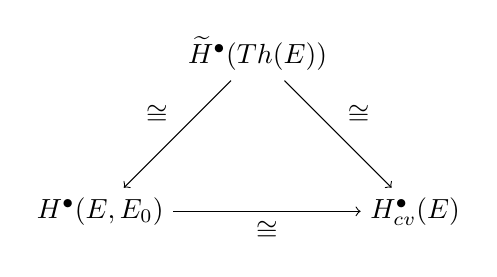
\begin{tikzpicture}[baseline=(current bounding box.east)]
                \node (TH) at (0, 0) {$\widetilde{H}^\bullet(\text{Th}(E))$};
                \node (R) at (-2, -2) {$H^\bullet(E, E_0)$};
                \node (CV) at (2, -2) {$H^\bullet_{cv}(E)$};
                \draw[->] (TH) -- node[above left]{$\cong$} (R);
                \draw[->] (TH) -- node[above right]{$\cong$} (CV);
                \draw[->] (R) -- node[below]{$\cong$} (CV);
            \end{tikzpicture}
        \end{gather}
    \end{property}

    \newdef{Thom spectrum}{\index{spectrum!Thom}
        Let $E\rightarrow M$ be a vector bundle. The Thom spectrum of $E$ is defined as the suspension spectrum of its Thom space. This can be written more explicitly as
        \begin{gather}
            (\Sigma^\infty\text{Th}(E))_n\cong\text{Th}(\mathbb{R}^n\oplus E)
        \end{gather}
        because of the existence of a homeomorphism $\text{Th}(\mathbb{R}^n\oplus E)\cong\Sigma^n\text{Th}(E)$.

        Let us now consider the sequence $\seq{\xi}$ of universal vector bundles. For every $\xi_n$ we define the $n^{th}$ component space as follows:
        \begin{gather}
            MO_n := \text{Th}(\xi_n).
        \end{gather}
        The Whitney sum $\xi_n\oplus\mathbb{R}$ can be obtained as a pullback of $\xi_{n+1}$. This map induces a map $\Sigma MO_n\rightarrow MO_{n+1}$, which gives the $n^{th}$ structure map of ''the'' Thom spectrum $MO$.\footnote{Note that the Thom spectrum as defined here is not an $\Omega$-spectrum \ref{topology:spectrum}, it is merely a sequential spectrum (prespectrum).}
    }

    \newdef{Euler class}{\index{Euler!class}
        Consider a vector bundle $E\rightarrow M$ together with its Thom class $\Phi$. The Euler class $e(E)$ is defined as the pullback $s_0^*\Phi$ of the Thom class along the zero section of $E$.
    }
    \begin{property}
        If the orientation of $E$ is reversed, the Euler class changes sign.
    \end{property}
    The following property distinguishes the Euler class among all characteristic classes of $E$:
    \begin{property}[Normalization]
        If the vector bundle admits a nowhere-vanishing section, its Euler class vanishes.
    \end{property}

\subsection{\v{C}ech-de Rham complex}\label{section:cech_de_rham}

    \begin{theorem}[Mayer-Vietoris sequence]\index{Mayer-Vietoris sequence}
        Consider a smooth manifold $M$ with an open covering $U\cup V$. The cohomology of $U,V$ is related to that of $M$ by the following short exact sequence:
        \begin{gather}
            0\longrightarrow H^\bullet(M)\longrightarrow H^\bullet(U)\oplus H^\bullet(V)\longrightarrow H^\bullet(U\cap V)\longrightarrow 0
        \end{gather}
        where the second arrow acts by restriction and the third one maps $(\omega,\rho)$ to $\rho-\omega$.
    \end{theorem}

    \newdef{\v{C}ech-de Rham complex}{
        Consider an open cover $\mathcal{U}=\{U_i\subseteq M\}_{i\in I}$ of a smooth manifold $M$.\footnote{Some authors require $I$ to be countable.} By $U_{i_0\ldots i_{k-1}}$ we denote the $k$-fold intersection $U_{i_0}\cap\cdots\cap U_{i_{k-1}}$. For all $k$ we define maps (where we suppress the label $k$) \[\delta_j:\Omega^\bullet(U_{i_0\ldots i_{k-1}})\rightarrow\prod_\alpha\Omega^\bullet(U_{i_0\ldots i_{j-1}\alpha i_j\ldots i_{k-1}})\] induced by the inclusions \[\iota_j:U_{i_0\ldots i_k}\hookrightarrow U_{i_0\ldots i_{j-1}i_{j+1}\ldots i_k}\] that ''ignore'' the $j^{th}$ open set. A total coboundary map $\delta$ is then defined as the alternating sum of the $\delta_i$'s:
        \begin{gather}
            (\delta\omega)_{i_0\ldots i_k} = \sum_{j=0}^k(-1)^i\omega_{i_0\ldots\widehat{i_j}\ldots i_k}
        \end{gather}
        for $\omega\in\prod\Omega^\bullet(U_{i_0\ldots i_{k-1}})$. It can be shown that $\delta$ is indeed a coboundary, i.e. $\delta^2=0$. The double complex $C^p(\mathcal{U}; \Omega^q):=\prod\Omega^q(U_{i_0\ldots i_p})$ with total differential $D=\delta+(-1)^pd$, where $d$ is the ordinary de Rham differential, is called the \v{C}ech-de Rham complex.
    }

    The Mayer-Vietoris sequence can be generalized to a statement for the \v{C}ech-de Rham complex:
    \begin{property}[Mayer-Vietoris sequence]
        The horizontal complex
        \begin{gather}
            0\longrightarrow\Omega^\bullet(M)\longrightarrow\prod_{i_0}\Omega^\bullet(U_{i_0})\longrightarrow\prod_{i_0,i_1}\Omega^\bullet(U_{i_0i_1})\longrightarrow\cdots
        \end{gather}
        is acyclic, i.e. the $\delta$-cohomology of the \v{C}ech-de Rham complex vanishes.
    \end{property}

    An important corollary is that one can compute the (de Rham) cohomology of $M$ using the above double complex:
    \begin{theorem}
        The restriction map $\Omega^\bullet(M)\rightarrow C^\bullet(\mathcal{U}; \Omega^\bullet)$ induces an isomorphism in cohomology.
    \end{theorem}
    One can also augment the \v{C}ech-de Rham complex in the other direction by the kernel of the de Rham differential in degree 1. These are the locally constant functions on the intersections $U_{i_0\ldots i_p}$. The cohomology of this augmenting sequence $C^\bullet(\mathcal{U}, \underline{\mathbb{R}})$ is called the \textbf{\v{C}ech cohomology} of $M$.\index{Cech!cohomology} By the same reason as for why the Mayer-Vietoris sequence implied the above theorem, we obtain the following theorem:
    \begin{theorem}[\v{C}ech $=$ de Rham]
        For a smooth manifold $M$, admitting a good cover $\mathcal{U}$, the \v{C}ech cohomology of $\mathcal{U}$ is isomorphic to the de Rham cohomology of $M$:
        \begin{gather}
            H^\bullet(M)\cong\check{H}^\bullet(\mathcal{U}; \underline{\mathbb{R}}).
        \end{gather}
    \end{theorem}
    \begin{result}
        All compact manifolds admit a finite good cover and hence have finite-dimensional de Rham cohomology.
    \end{result}

    We will now construct a generalization of \v{C}ech cohomology. The notation $\underline{\mathbb{R}}$ above should remind us of example \ref{sheaf:constant_sheaf}, i.e. $\underline{\mathbb{R}}$ denotes the sheaf of locally constant functions with values in $\mathbb{R}$. Similarly $\Omega^\bullet$ should be regarded as the sheaf of differential forms.
    \newdef{\v{C}ech cohomology}{\index{Cech!cohomology}
        Let $\mathcal{F}$ be a (pre)sheaf of Abelian groups. For an open cover $\mathcal{U}=\{U_i\subseteq M\}_{i\in I}$ we define the cochain groups
        \begin{gather}
            C^p(\mathcal{U};\mathcal{F}) := \prod_{i_0<\cdots<i_p}\mathcal{F}(U_{i_0\ldots i_p})
        \end{gather}
        for all $p\in\mathbb{N}$ as before. Since the (pre)sheaf takes values in Abelian groups we can define the subtraction of elements and hence the definition of the differential $\delta$ still makes sense:
        \begin{gather}
            \delta := \sum_{i=0}^k(-1)^i\mathcal{F}(\iota_i)
        \end{gather}
        where $\iota_i$ are the inclusion maps as before. The $\delta$-cohomology of the complex $C^\bullet(\mathcal{U}; \mathcal{F})$ is called the \v{C}ech cohomology of $\mathcal{U}$ with values in $\mathcal{F}$.

        By taking the direct limit over the direct system of open covers of a smooth manifold $M$ (the partial ordering is given by refinement of covers) one can define the \v{C}ech cohomology $\check{H}^\bullet(M; \mathcal{F})$ of $M$ with values in $\mathcal{F}$.
    }

    By noting that good covers are \textit{cofinal} in the set of open covers one can obtain the following theorem:
    \begin{theorem}[\v{C}ech $=$ de Rham, bis]
        For a smooth manifold the \v{C}ech cohomology of $M$ with values in $\underline{\mathbb{R}}$ is isomorphic to the de Rham cohomology of $M$:
        \begin{gather}
            H^\bullet(M)\cong\check{H}^\bullet(M;\underline{\mathbb{R}}).
        \end{gather}
    \end{theorem}

    \begin{example}[Zeroth cohomology]
        From the general definition of cohomology groups and the specific form of the coboundary operator we find that \[\omega_{\alpha_0}|_{U_{\alpha_0}\cap U_{\alpha_1}}=\omega_{\alpha_1}|_{U_{\alpha_0}\cap U_{\alpha_1}}\] for all $\alpha_0\neq\alpha_1$ and $\omega\in\check{H}^0(M;\mathcal{F})$. This is exactly the defining relation for the (global) sections of $\mathcal{F}$ and hence we obtain (as usual)
        \begin{gather}
            \check{H}^0(M;\mathcal{F})\cong\mathcal{F}(M).
        \end{gather}
    \end{example}

\subsection{Non-orientable manifolds}

    \newdef{Twisted cohomology}{\index{cohomology!twisted}
        Let $E\rightarrow M$ be a flat vector bundle over $M$. By construction \ref{diff:twisted_differential} we know that the algebra $\Omega^\bullet(M)\otimes E$ can be given the structure of a differential graded algebra \ref{linalgebra:dg_algebra} and hence gives rise to a cohomology theory $H^\bullet(M; E)$. This is called the $E$-twisted de Rham cohomology of $M$.
    }
    \begin{remark}
        By the remark following construction \ref{diff:twisted_differential} we should pay attention to what trivialization was used in the construction of $H^\bullet(M; E)$. It can be shown that two trivializations give rise to the same $E$-twisted cohomology if they admit a common refinement for which the induced sections differ by a locally constant matrix $a\in\text{GL}(n, \mathbb{R})$.
    \end{remark}

    If we take $E=o(M)$ to be the orientation line bundle over $M$, we obtain the (honest) densities of remark \ref{diff:honest_density}. The cohomology of this complex is simply called the \textbf{twisted de Rham cohomology}.
    \begin{property}[Isomorphisms]
        The twisted cohomologies defined by two trivializations induced from atlases on $M$ are isomorphic.\footnote{Although we almost always work with natural trivialization, i.e. where the open subsets of $M$ are obtained from charts on $M$, this is not technically necessary. For these ''exotic'' cases, the isomorphisms not always exist.}
    \end{property}
    \begin{property}[Trivial twisting]
        If $M$ is orientable, its twisted cohomology is isomorphic to its ordinary (de Rham) cohomology. More generally, the $E$-twisted de Rham cohomology is isomorphic to the ordinary de Rham cohomology whenever $E$ is trivial.
    \end{property}

    Poincar\'e duality \ref{diff:poincare_duality} can be translated almost verbatim to the twisted case:
    \begin{theorem}[Poincar\'e duality]\index{Poincar\'e!duality}
        Integration of densities induces the following isomorphism:
        \begin{gather}
            H^k(M)\cong\left(H^{m-k}_c(M; o(M))\right)^*.
        \end{gather}
        If $M$ is of finite type, the converse also holds:
        \begin{gather}
            H^k_c(M)\cong\left(H^{m-k}(M; o(M))\right)^*.
        \end{gather}
    \end{theorem}
    The Thom isomorphism also holds for non-orientable bundles:
    \begin{theorem}[Thom isomorphism]\index{Thom!isomorphism}
        Let $E\rightarrow M$ be a rank-$n$ vector bundle. Fibre integration gives the following isomorphism:
        \begin{gather}
            H^{\bullet+n}_{cv}(E)\cong H^\bullet(M; o(E)).
        \end{gather}
    \end{theorem}

\section{Differential operators}

    In this section the study of PDEs is generalized to vector bundles. The case of PDEs on $\mathbb{R}^n$ was treated in chapter \ref{chapter:pde}.

    \newdef{Differential operator}{\index{differential!operator}\index{elliptic!operator}
        A (linear) differential operators between two vector bundels $E,F$ over the same base manifold $X$ is a linear map $\Gamma(E)\rightarrow\Gamma(F)$ that can locally be expressed as a system of partial differential equations.

        The principal symbol of this operator is defined as the principal symbol \ref{pde:principal_symbol} of the associated PDE. By extension one says the differential operator is \textbf{elliptic} (hyperbolic, \ldots) if its associated PDE is elliptic (hyperbolic, \ldots).
    }

    \newdef{Normally hyperbolic operators}{\index{hyperbolic}
        Consider a (pseudo)Riemannian vector bundle $E$ (see chapter \ref{chapter:riemann}). A linear differential operator on $E$ is said to be normally hyperbolic if its principal symbol is proportional to the given metric.
    }

\subsection{Elliptic complexes}

    \newdef{Elliptic complex}{
        Consider a collection of vector bundles $\{\pi_i:E_i\rightarrow M\}_{i\in\mathbb{N}}$ together with a collection of differential operators $\{D_i:C^\infty(E_i)\rightarrow C^\infty(E_{i+1})\}_{i\in\mathbb{N}}$. This system is called an elliptic complex if it is a cochain complex, i.e. $D_{i+1}\circ D_i = 0$, and if the induced sequence $\{\sigma_p(\xi)(D_i)\}_{i\in\mathbb{N}}$ is exact for all $x\in M$ and $\xi\neq0$.
    }

    ?? COMPLETE ??

\section{Linear connections}\label{section:linear_connections}

    \newdef{Koszul connection}{\index{connection!Koszul}\label{diff:koszul_connection}
        Let $\pi: E\rightarrow M$ be a vector bundle over a smooth manifold $M$. A Koszul connection (or \textbf{linear connection)} on $E$ is a (smooth) linear map $\nabla:\Gamma(E)\rightarrow\Gamma(T^*M\otimes E)$ satisfying the Leibniz property
        \begin{gather}
            \nabla(f\sigma) = f\nabla\sigma + df\otimes\sigma
        \end{gather}
        for all $f\in C^\infty(M)$.
    }
    \begin{property}
        Because $\nabla\sigma$ takes a vector field as input, which is a $C^\infty(M)$-linear operation, the connection satisfies the following linearity property:
        \begin{gather}
            \nabla_{fX + Y}\sigma = f\nabla_X\sigma + \nabla_Y\sigma.
        \end{gather}
    \end{property}

    \begin{formula}
        Let $E, E'$ be two vector bundles over the same manifold $M$. Koszul connections on $E$ and $E'$ induce a connection on the tensor product bundle $E\otimes E'$ as follows:
        \begin{gather}
            \nabla(X\otimes Y) := \nabla X\otimes Y + X\otimes\nabla Y
        \end{gather}
        for $X\in\Gamma(E), Y\in\Gamma(E')$.
    \end{formula}

    \begin{example}[Affine connection]\index{connection!affine}
        Let $M$ be a smooth manifold. An affine connection $\nabla:\mathfrak{X}(M)\times\mathfrak{X}(M)\rightarrow \mathfrak{X}(M)$ is a Koszul connection on the tangent bundle.
    \end{example}

    \begin{property}[Local behaviour]
        Consider a vector $v\in T_pM$. If two vector fields $X, Y\in \Gamma(TM)$ are equal on some neighbourhood $U$ of $p$, then $\nabla_vX = \nabla_vY$ at $p$. Furthermore, given a curve $c:[0, 1]\rightarrow M$ and two vector fields $X, Y\in\Gamma(TM)$ such that $X\circ c = Y\circ c$ one finds that $\nabla_{\dot c}X = \nabla_{\dot c}Y$. This implies that an affine connection only depends on the local behaviour of the given section.
    \end{property}
    \begin{remark}
        The above property shows the major difference between the Lie derivative and the covariant derivative when acting on sections of the tangent bundle $\sigma$. Lie derivatives depend on the local behaviour of both $X$ and $\sigma$. The covariant derivative on the other hand only depends on the value of $X$ at $p\in M$ and on the local behaviour of $\sigma$.
    \end{remark}

    \begin{property}[Affinity]
        Consider two affine connections $\nabla, \overline\nabla$ on a smooth manifold $M$. The operator $\nabla-\overline\nabla$ is an endormorphism of $E$, i.e. $\nabla-\overline\nabla\in\Omega^1(M;\text{End}(E))$. It follows that the set of affine connections forms an affine space (hence the name).
    \end{property}

    \newdef{Parallel tensor fields}{\index{parallel}
        A tensor field $T$ is said to be parallel with respect to a connection $\nabla$ if it satisfies $\nabla T = 0$. It is said to be parallel with respect to a vector field $X$ if $\nabla_XT = 0$.
    }
    \begin{example}
        Important examples in the case of the Levi-Civita connection on a Riemannian manifold are the volume form Vol and the metric $g$ (Chapter \ref{chapter:riemann}).
    \end{example}

    \newdef{Connection coefficients}{\index{Christoffel symbols}\label{diff:christoffel_symbol}
        Let $E$ be a smooth rank-$k$ vector bundle. Consider a Koszul connection $\nabla$, a (local) frame $\{e_i\}_{1\leq i\leq k}$ and a (local) coframe $\{f^i\}_{1\leq i\leq k}$ on $E$. For every vector field $e_i$ one can (locally) write
        \begin{gather}
            \nabla e_i = \Gamma^k_{\ ji}e_k\otimes f^j.
        \end{gather}
        The quantities $\Gamma^k_{\ ji}$ are called the connection coefficients or \textbf{Christoffel symbols} of $\nabla$. For a general vector field $\sigma = \sigma^ie_i$ one then obtains (if $\{e_i,f^i\}_{1\leq i\leq k}$ are coordinate-induced):
        \begin{align}
            \nabla\sigma &= (\nabla\sigma^i)\otimes e_i + \sigma^i(\nabla e_i)\nonumber\\
            &= (\partial_j\sigma^k)e_k\otimes f^j + \sigma^i(\Gamma^k_{\ ji}e_k\otimes f^j)\nonumber\\
            &= (\partial_j\sigma^k + \Gamma^k_{\ ji}\sigma^i)e_k\otimes f^j.
        \end{align}
    }

\subsection{Induced connections}

    \begin{formula}[Connection on tensors]
        Applying the Leibniz property of a Koszul connection to tensor contractions gives us the following form of the induced connection on the $(k,l)$-tensor bundle:
        \begin{align}
            \nabla_YT(\omega^1,\ldots,\omega^k,X_1,\ldots,X_l) := Y\Big(&T(\omega^1,\ldots,\omega^k,X_1,\ldots,X_l)\Big)\nonumber\\
            &- \sum_{i=1}^kT(\omega^1,\ldots,\nabla_Y\omega^i,\ldots,\omega^k,X_1,\ldots,X_l)\nonumber\\
            &- \sum_{i=1}^lT(\omega^1,\ldots,\omega^l,X_1,\ldots,\nabla_YX_i,\ldots,X_l)
        \end{align}
        where $Y,X_1,\ldots,X_l\in\mathfrak{X}(M)$ and $\omega^1,\ldots,\omega^k\in\Omega^1(M)$.
    \end{formula}

    \begin{result}
        By noting that the covariant derivative of a vector field is a vector-valued differential form, one can use the previous formula to compute the covariant derivative of the covariant derivative:
        \begin{gather}
            (\nabla_X\nabla)_YZ = \nabla_X(\nabla_YZ) - \nabla_{\nabla_XY}Z - \nabla_Y(\nabla_XZ).
        \end{gather}
        Parentheses were added to make it clear that the outer covariant derivatives act on the result of the inner derivatives. If these parentheses would not have been added, these terms could have been confused with the second covariant derivative (whose definition also follows from a Leibniz-type argument):
        \begin{gather}
            \nabla^2_{X,Y}S : = \nabla_X(\nabla_YS) - \nabla_{\nabla_XY}S.
        \end{gather}
    \end{result}

    As an example of the second covariant derivative the definition of the Hessian on arbitrary smooth manifolds is given:
    \newdef{Hessian}{\index{Hessian}
        Consider a smooth manifold with connection $\nabla$. The Hessian of a function $f\in C^\infty(M)$ is defined as the iterated covariant derivative:
        \begin{gather}
            \text{Hess}(f) := \nabla^2f
        \end{gather}
        where one should note that by the above definition the first covariant derivative also acts on the second one, i.e\mnote{\dbend}
        \begin{gather}
            \nabla^2f(X,Y) = \nabla_X(\nabla_Yf) - \nabla_{\nabla_XY}f.
        \end{gather}
        For a scalar function one knows that $\nabla f = df$ and for covector fields one knows that (in local coordinates) \[\nabla_i\sigma_j = \partial_i\sigma_j - \Gamma^k_{ij}\sigma_k\] where $\Gamma^k_{ij}$ are the connection coefficients. Combining these facts one obtains the following local formula for the Hessian of $f$:
        \begin{gather}
            \text{Hess}(f) = \left(\frac{\partial^2f}{\partial x_i\partial x_j} - \Gamma^k_{ij}\pderiv{f}{x_k}\right)dx^i\otimes dx^j.
        \end{gather}
    }

    \newdef{Pullback connection}{\index{connection!pullback}
        Let $E\rightarrow N$ be a vector bundle with Koszul connection $\nabla$ and let $f:M\rightarrow N$ be a smooth map. On the pullback bundle \ref{diff:pullback_bundle} there exists a unique Koszul connection $\nabla'$ satisfying
        \begin{gather}
            \nabla'(f^*\chi) = f^*(\nabla\chi)
        \end{gather}
        for any section $\chi$ of $E$.
    }
    \newdef{Invariant connection}{\index{connection!invariant}
        Let $G$ be a Lie group acting on a vector bundle $E\rightarrow M$. A Koszul connection $\nabla$ on $E$ is said to be invariant with respect to the $G$-action if it satisfies:
        \begin{gather}
            g^*\nabla = \nabla
        \end{gather}
        for all $g\in G$.
    }